\section{Related Work}
% Sec 2.1. Review of previous work (i.e. previous methods that have explored a similar problem)
% Sec 2.2. Say why your method is better than previous work; and/or summarize the key main contributions of your work;
\subsection{StyleGan}

\subsection{Human Pose}
There are many existing work focusing on human pose estimation, such as yolo \cite{yolo1} \cite{yolo2} \cite{yolo3} \cite{wang2022yolov7}. However, we find that if we inference on our laptop, it'll run very slow. The FPS of the game will drop to 2 or 3, which is unsuitable for our application. What we need is a simple backbone that can perform human pose estimation real-time, instead of a heavy backbone that can predict very accurately.

Therefore, we search for a simple network that satisfies our goal and we find \textbf{mediapipe} \cite{lugaresi2019mediapipe}. We find that it can perform human pose estimation real-time mainly due to two reasons. First, Figure \ref{fig:yolo_arch} and Figure \ref{fig:mp_arch} shows the architecture of YOLOv7 and mediapipe respectively. We can easily find that the architecture of YOLOv7 is far more complicated than that of mediapipe. We can infer that the number of parameters in mediapipe is far less than that in YOLOv7, so the inference speed may be faster.

\begin{figure}[ht]
    \centering
    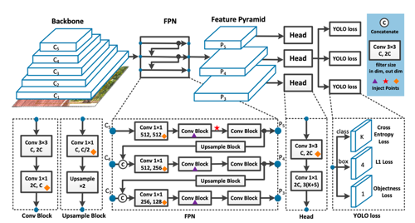
\includegraphics[scale=.55]{fig/yolo_arch.png}
    \caption{Architecture of YOLOv7 \cite{wang2022yolov7}.}
    \label{fig:yolo_arch}
\end{figure}

\begin{figure}[ht]
    \centering
    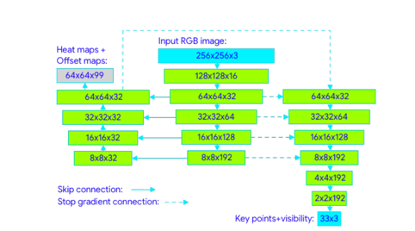
\includegraphics[scale=.6]{fig/mp_arch.png}
    \caption{Architecture of Mediapipe \cite{lugaresi2019mediapipe}.}
    \label{fig:mp_arch}
\end{figure}

The original version of mediapipe, however, only supports human pose estimation for single person, but our game definitely requires the simultaneous huamn pose estimation on two people. Therefore, we make some modification to it, which will be elaborated in \ref{mediapipework}.

\subsection{game inference}